\section{Results}
\label{sec:results}
\subsection{Frequency of Utilizations in Python Projects}
\subsubsection{Saturation of Projects with Utilizations}
Out of the \DTLfetch{data}{key}{nProjScanned}{value}\ projects scanned, \DTLfetch{data}{key}{percentProjectsUsingRegex}{value}\% (\DTLfetch{data}{key}{nProjectsUsingRegex}{value}) contained at least one utilization.  For context about how saturated these projects were with utilizations, we consider how many utilizations were observed per project, how many files the average project scanned contained, how many of those files contained utilizations, and how many utilizations occurred per file in table~\ref{table:contextHistogram}.

\begin{table}[tb]
\caption{How saturated are projects with utilizations? (RQ1)}
\label{table:contextHistogram}
\begin{center}
\begin{center}
\begin{tabular}{l|ccccc}
\toprule
source & Q1 & Avg & Med & Q3 & Max \\ 
\midrule
files per project & 2 & 53 & 6 & 21 & 5,963 \\ 
\midrule
files with regex per project & 1 & 11 & 2 & 6 & 541 \\ 
\midrule
regex usages per file & 1 & 2 & 1 & 3 & 207 \\ 
\bottomrule
\end{tabular}
\end{center}

\end{center}
\end{table}

\subsubsection{Usage Frequency of {\tt re} Module Functions and Flags}

\begin{figure}[tb]
\centering
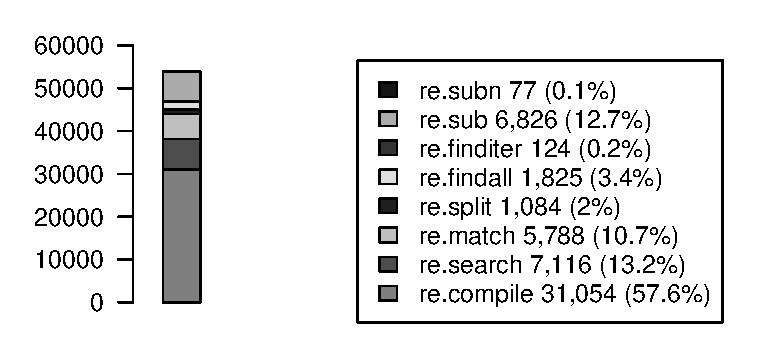
\includegraphics[width=\columnwidth]{../analysis_output/partFunctions.eps}
\caption{How often are the 8 re functions used? (RQ1)}
\label{fig:partFunctions}
\end{figure}

As seen in Figure~\ref{fig:partFunctions} The `compile' function encompasses \DTLfetch{data}{key}{percentCompile}{value}\% of all utilizations, presumably because each usage of those functions could accept the compiled regex as an argument.

\begin{figure}[tb]
\centering
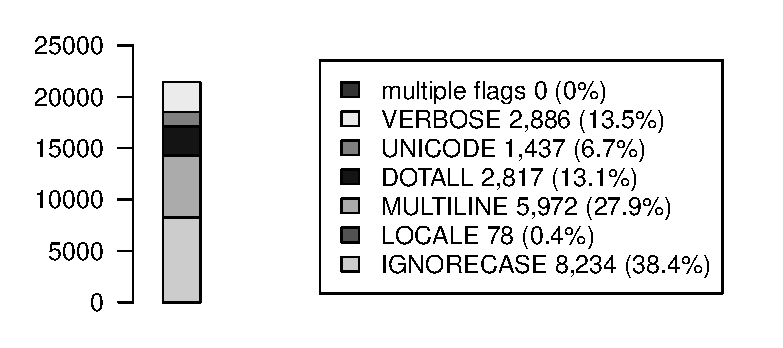
\includegraphics[width=\columnwidth]{../analysis_output/partFlags.eps}
\caption{Which behavioral flags are used? (RQ1)}
\label{fig:partFlags}
\end{figure}

When considering flag use, we excluded non-behavioral flags (default and debug), which account for \DTLfetch{data}{key}{percentFlags0}{value}\% of all utilizations.

 As shown in figure ~\ref{fig:partFlags}, of all behavioral flags used, ignorecase (\DTLfetch{data}{key}{percentI}{value}\%) and multiline (\DTLfetch{data}{key}{percentM}{value}\%) were the most frequently used.  It is also worth noting that although multiple flags can be combined using a bitwise or, this was never observed.

\todo{top regex patterns go here}

\todo{topNW table?}
% \subsubsection{{General Characteristics of Regexes Found}}
% \todo{could the top 10 regexes be a pop-out?}
% \begin{table}
\caption{ \label{}}
\begin{center}
\begin{tabular}{lc}
\toprule
pattern & weight \\ 
\midrule
\begin{minipage}{2.3in}
\begin{verbatim}
'\\s+'\end{verbatim}
\end{minipage}
& 181 \\ 
\midrule
\begin{minipage}{2.3in}
\begin{verbatim}
'\\s'\end{verbatim}
\end{minipage}
& 78 \\ 
\midrule
\begin{minipage}{2.3in}
\begin{verbatim}
'\\d+'\end{verbatim}
\end{minipage}
& 70 \\ 
\midrule
\begin{minipage}{2.3in}
\begin{verbatim}
'[\\x80-\\xff]'\end{verbatim}
\end{minipage}
& 69 \\ 
\midrule
\begin{minipage}{2.3in}
\begin{verbatim}
'\nmd5_data = {\n([^}]+)}'\end{verbatim}
\end{minipage}
& 69 \\ 
\midrule
\begin{minipage}{2.3in}
\begin{verbatim}
'\\\\(.)'\end{verbatim}
\end{minipage}
& 67 \\ 
\midrule
\begin{minipage}{2.3in}
\begin{verbatim}
'([\\\\"]|[^\\ -~])'\end{verbatim}
\end{minipage}
& 66 \\ 
\midrule
\begin{minipage}{2.3in}
\begin{verbatim}
'(-?(?:0|[1-9]\\d*))(\\.\\d+)?([eE][-+]?\\d+)?'\end{verbatim}
\end{minipage}
& 61 \\ 
\midrule
\begin{minipage}{2.3in}
\begin{verbatim}
'[^]]+?\\] +([0-9.]+): (\\w+) <-(\\w+)'\end{verbatim}
\end{minipage}
& 60 \\ 
\midrule
\begin{minipage}{2.3in}
\begin{verbatim}
'.*rlen=([0-9]+)'\end{verbatim}
\end{minipage}
& 57 \\ 
\bottomrule
\end{tabular}
\end{center}
\end{table}


\subsection{Frequency of Feature Usage}

Literal tokens were found in \DTLfetch{data}{key}{P_LITERAL_PRESENT}{value}\% of patterns, and accounted for \DTLfetch{data}{key}{P_LITERAL_TOKENS}{value}\% of all tokens.  We consider literal tokens to be ubiquitous in all utilizations, and necessary for any regex related tool, and so exclude them from the rest of the feature analysis.  In table~\ref{table:featureStats}, we display a large body of information about feature usage and relate it to four major regex related projects.

\begin{table*}[h]
\begin{center}
\begin{small}
\caption{How Frequently do Features Appear in Projects? (RQ2)}
\label{table:featureStats}
\begin{tabular}
{ll@{ }llc@{ }c@{ }c@{ }ccccccc}
rank & code & description & example & brics & hampi & Rex & RE2 & nPatterns & \% patterns & nProjects & \% projects \\ 
\toprule[0.16em]
1 & ADD & one-or-more repetition & \begin{minipage}{0.5in}\begin{verbatim}z+\end{verbatim}\end{minipage} & \yes & \yes & \yes & \yes & 6,003 & 44.1 & 1,204 & 73.2 \\ 
\midrule
2 & CG & a capture group & \begin{minipage}{0.5in}\begin{verbatim}(caught)\end{verbatim}\end{minipage} & \yes & \yes & \yes & \yes & 7,130 & 52.4 & 1,194 & 72.6 \\ 
\midrule
3 & KLE & zero-or-more repetition & \begin{minipage}{0.5in}\begin{verbatim}.*\end{verbatim}\end{minipage} & \yes & \yes & \yes & \yes & 6,017 & 44.3 & 1,099 & 66.8 \\ 
\midrule
4 & CCC & custom character class & \begin{minipage}{0.5in}\begin{verbatim}[aeiou]\end{verbatim}\end{minipage} & \yes & \yes & \yes & \yes & 4,468 & 32.9 & 1,026 & 62.4 \\ 
\midrule
5 & ANY & any non-newline char & \begin{minipage}{0.5in}\begin{verbatim}.\end{verbatim}\end{minipage} & \yes & \yes & \yes & \yes & 4,657 & 34.3 & 1,005 & 61.1 \\ 
\midrule
6 & RNG & chars within a range & \begin{minipage}{0.5in}\begin{verbatim}[a-z]\end{verbatim}\end{minipage} & \yes & \yes & \yes & \yes & 2,631 & 19.3 & 848 & 51.6 \\ 
\midrule
7 & STR & start-of-line & \begin{minipage}{0.5in}\begin{verbatim}^\end{verbatim}\end{minipage} & \no & \yes & \yes & \yes & 3,563 & 26.2 & 846 & 51.4 \\ 
\midrule
8 & END & end-of-line & \begin{minipage}{0.5in}\begin{verbatim}$\end{verbatim}\end{minipage} & \no & \yes & \yes & \yes & 3,169 & 23.3 & 827 & 50.3 \\ 
\midrule[0.12em]
9 & NCCC & negated CCC & \begin{minipage}{0.5in}\begin{verbatim}[^qwxf]\end{verbatim}\end{minipage} & \yes & \yes & \yes & \yes & 1,935 & 14.2 & 776 & 47.2 \\ 
\midrule
10 & WSP & \textbackslash t \textbackslash n \textbackslash r \textbackslash v \textbackslash f or space & \begin{minipage}{0.5in}\begin{verbatim}\s\end{verbatim}\end{minipage} & \no & \yes & \yes & \yes & 2,846 & 20.9 & 762 & 46.3 \\ 
\midrule
11 & OR & logical or & \begin{minipage}{0.5in}\begin{verbatim}a|b\end{verbatim}\end{minipage} & \yes & \yes & \yes & \yes & 2,102 & 15.5 & 708 & 43 \\ 
\midrule
12 & DEC & any of: 0123456789 & \begin{minipage}{0.5in}\begin{verbatim}\d\end{verbatim}\end{minipage} & \no & \yes & \yes & \yes & 2,297 & 16.9 & 692 & 42.1 \\ 
\midrule
13 & WRD & [a-zA-Z0-9\_] & \begin{minipage}{0.5in}\begin{verbatim}\w\end{verbatim}\end{minipage} & \no & \yes & \yes & \yes & 1,430 & 10.5 & 650 & 39.5 \\ 
\midrule
14 & QST & zero-or-one repetition & \begin{minipage}{0.5in}\begin{verbatim}z?\end{verbatim}\end{minipage} & \yes & \yes & \yes & \yes & 1,871 & 13.8 & 645 & 39.2 \\ 
\midrule
15 & LZY & as few reps as possible & \begin{minipage}{0.5in}\begin{verbatim}z+?\end{verbatim}\end{minipage} & \no & \yes & \no & \yes & 1,300 & 9.6 & 605 & 36.8 \\ 
\midrule
16 & NCG & group without capturing & \begin{minipage}{0.5in}\begin{verbatim}a(?:b)c\end{verbatim}\end{minipage} & \no & \yes & \no & \yes & 791 & 5.8 & 404 & 24.6 \\ 
\midrule
17 & PNG & named capture group & \begin{minipage}{0.5in}\begin{verbatim}(?P<name>x)\end{verbatim}\end{minipage} & \no & \yes & \no & \yes & 915 & 6.7 & 354 & 21.5 \\ 
\midrule
18 & SNG & exactly n repetition & \begin{minipage}{0.5in}\begin{verbatim}z{8}\end{verbatim}\end{minipage} & \yes & \yes & \yes & \yes & 581 & 4.3 & 340 & 20.7 \\ 
\midrule
19 & NWSP & any non-whitespace & \begin{minipage}{0.5in}\begin{verbatim}\S\end{verbatim}\end{minipage} & \no & \yes & \yes & \yes & 484 & 3.6 & 270 & 16.4 \\ 
\midrule
20 & DBB & $n\le x \le m$ repetition & \begin{minipage}{0.5in}\begin{verbatim}z{3,8}\end{verbatim}\end{minipage} & \yes & \yes & \yes & \yes & 367 & 2.7 & 238 & 14.5 \\ 
\midrule
21 & NLKA & sequence doesn't follow  & \begin{minipage}{0.5in}\begin{verbatim}a(?!yz)\end{verbatim}\end{minipage} & \no & \no & \no & \no & 131 & 1 & 183 & 11.1 \\ 
\midrule
22 & WNW & word/non-word boundary & \begin{minipage}{0.5in}\begin{verbatim}\b\end{verbatim}\end{minipage} & \no & \no & \no & \yes & 248 & 1.8 & 166 & 10.1 \\ 
\midrule
23 & NWRD & non-word chars & \begin{minipage}{0.5in}\begin{verbatim}\W\end{verbatim}\end{minipage} & \no & \yes & \yes & \yes & 94 & 0.7 & 165 & 10 \\ 
\midrule
24 & LWB & at least n repetition & \begin{minipage}{0.5in}\begin{verbatim}z{15,}\end{verbatim}\end{minipage} & \yes & \yes & \yes & \yes & 91 & 0.7 & 158 & 9.6 \\ 
\midrule
25 & LKA & matching sequence follows & \begin{minipage}{0.5in}\begin{verbatim}a(?=bc)\end{verbatim}\end{minipage} & \no & \no & \no & \no & 112 & 0.8 & 158 & 9.6 \\ 
\midrule
26 & OPT & options wrapper & \begin{minipage}{0.5in}\begin{verbatim}(?i)CasE\end{verbatim}\end{minipage} & \no & \yes & \no & \yes & 231 & 1.7 & 154 & 9.4 \\ 
\midrule
27 & NLKB & sequence doesn't precede & \begin{minipage}{0.5in}\begin{verbatim}(?<!x)yz\end{verbatim}\end{minipage} & \no & \no & \no & \no & 94 & 0.7 & 137 & 8.3 \\ 
\midrule[0.12em]
28 & LKB & matching sequence precedes & \begin{minipage}{0.5in}\begin{verbatim}(?<=a)bc\end{verbatim}\end{minipage} & \no & \no & \no & \no & 80 & 0.6 & 120 & 7.3 \\ 
\midrule
29 & ENDZ & absolute end of string & \begin{minipage}{0.5in}\begin{verbatim}\Z\end{verbatim}\end{minipage} & \no & \no & \no & \yes & 89 & 0.7 & 90 & 5.5 \\ 
\midrule
30 & BKR & match the $i^{th}$ CG & \begin{minipage}{0.5in}\begin{verbatim}\1\end{verbatim}\end{minipage} & \no & \no & \no & \no & 60 & 0.4 & 84 & 5.1 \\ 
\midrule
31 & NDEC & any non-decimal & \begin{minipage}{0.5in}\begin{verbatim}\D\end{verbatim}\end{minipage} & \no & \yes & \yes & \yes & 36 & 0.3 & 58 & 3.5 \\ 
\midrule
32 & BKRN & references PNG & \begin{minipage}{0.5in}\begin{verbatim}\g<name>\end{verbatim}\end{minipage} & \no & \yes & \no & \no & 17 & 0.1 & 28 & 1.7 \\ 
\midrule
33 & VWSP & matches U+000B & \begin{minipage}{0.5in}\begin{verbatim}\v\end{verbatim}\end{minipage} & \no & \no & \yes & \yes & 13 & 0.1 & 15 & 0.9 \\ 
\midrule
34 & NWNW & negated WNW & \begin{minipage}{0.5in}\begin{verbatim}\B\end{verbatim}\end{minipage} & \no & \no & \no & \yes & 4 & 0 & 11 & 0.7 \\ 
\bottomrule[0.13em]
\end{tabular}
\end{small}
\end{center}
\vspace{-12pt}
\end{table*}

%note captions and label are in external file
% use:\label{table:featureStats}

\subsection{Features Usage Analysis}
\subsubsection{Behavioral Clustering Results Overview}

% TODO - multiple boxplots for all 5-6 demonstrating cluster size and then also have \# of clusters, pick smallest number of clusters and then use that.
%(I think it's more complicated than that, perhaps we can link to my discussion about how I explored the space to find the best i, p, k values)

Our behavioral clustering technique found 952 clusters over 2727 patterns, with at least one cluster present in 999 of the 9727 projects that were compatible with Rex.

\todo{Need to know why MCL is behaving like this}

Table~\ref{table:exampleCluster} provides an example of a smaller behavioral cluster, representing 13 patterns, with at least one pattern from this cluster present in 100 different projects.

\begin{table}
\begin{center}
\caption{Sample from an example cluster (RQ4)}
\label{table:exampleCluster}
\begin{small}
\begin{tabular}
{lcc | lcc}
\toprule
index & pattern & nProjects & index & pattern & nProjects \\
 \hline \bigstrut
1 & \begin{minipage}{0.3in}\begin{verbatim}`:+'\end{verbatim}\end{minipage} & 8 & 5 & \begin{minipage}{0.5in}\begin{verbatim}`[:]'\end{verbatim}\end{minipage} & 6 \\
 \hline \bigstrut
2 & \begin{minipage}{0.3in}\begin{verbatim}`(:)'\end{verbatim}\end{minipage} & 8 & 6 & \begin{minipage}{0.6in}\begin{verbatim}`([^:]+):(.*)'\end{verbatim}\end{minipage} & 6 \\
 \hline \bigstrut
3 & \begin{minipage}{0.3in}\begin{verbatim}`(:+)'\end{verbatim}\end{minipage} & 8 & 7 & \begin{minipage}{0.5in}\begin{verbatim}`\s*:\s*'\end{verbatim}\end{minipage} & 4 \\
 \hline \bigstrut
4 & \begin{minipage}{0.3in}\begin{verbatim}`(:)(:*)'\end{verbatim}\end{minipage} & 8 & 8 & \begin{minipage}{0.5in}\begin{verbatim}`\:'\end{verbatim}\end{minipage} & 2 \\
\bottomrule
\end{tabular}
\vspace{-6pt}
\end{small}
\end{center}
\end{table}


%
%\begin{table}
%\begin{center}
%\caption{An example cluster (RQ3)}
%\label{table:exampleCluster}
%\begin{small}
%\begin{tabular}
%{lcc}
%\toprule
%index & pattern & nProjects\\
%\midrule
%1 & \begin{minipage}{0.5in}\begin{verbatim}`\s*,\s*'\end{verbatim}\end{minipage} & 54  \\
%\midrule
%2 & \begin{minipage}{0.5in}\begin{verbatim}`,'\end{verbatim}\end{minipage} & 30 \\
%\midrule
%3 & \begin{minipage}{0.5in}\begin{verbatim}`\s*,'\end{verbatim}\end{minipage} & 16 \\
%\midrule
%4 & \begin{minipage}{0.5in}\begin{verbatim}` ,\s*'\end{verbatim}\end{minipage} & 13 \\
%\midrule
%5 & \begin{minipage}{0.5in}\begin{verbatim}` *, *'\end{verbatim}\end{minipage} & 12 \\
%\midrule
%6 & \begin{minipage}{0.5in}\begin{verbatim}`,\S'\end{verbatim}\end{minipage} & 5 \\
%\midrule
%7 & \begin{minipage}{0.5in}\begin{verbatim}`,.*$'\end{verbatim}\end{minipage} & 3 \\
%\midrule
%8 & \begin{minipage}{0.6in}\begin{verbatim}`(\S+)\s*,\s*'\end{verbatim}\end{minipage} & 2 \\
%\midrule
%9 & \begin{minipage}{0.5in}\begin{verbatim}`,+'\end{verbatim}\end{minipage} & 1 \\
%\midrule
%10 & \begin{minipage}{0.5in}\begin{verbatim}`,\ ?'\end{verbatim}\end{minipage} & 1 \\
%\midrule
%10 & \begin{minipage}{0.5in}\begin{verbatim}`,\s*(\S)'\end{verbatim}\end{minipage} & 1 \\
%\midrule
%11 & \begin{minipage}{0.5in}\begin{verbatim}`\s*(,)\s*'\end{verbatim}\end{minipage} & 1 \\
%\midrule
%12 & \begin{minipage}{0.5in}\begin{verbatim}`\s*\,\s*'\end{verbatim}\end{minipage} & 1 \\
%\bottomrule
%\end{tabular}
%\end{small}
%\end{center}
%\end{table}

On first glance this cluster may seem to revolve around the `\verb!\s*!' parts of these patterns, but actually this cluster was formed because each of these patterns has a comma literal, and other details did not interfere with matching the Rex-generated strings with commas in them.

It is not a coincidence that the smallest pattern in this cluster gives the best idea of what all the patterns within it have in common (the smallest pattern is just the single comma character, at index 1).  All of the clusters we found follow this trend: the shortest pattern describes the rest of the pattern's behavior very well.  In table~\ref{table:topNClusters}, I show the top 10 clusters, ranked by the number of projects they appear in, using the shortest pattern from the cluster as an example.
The cluster in Table~\ref{table:exampleCluster} appears in the seventh row of Table~\ref{table:topNClusters}.

\begin{center}
\begin{table}
\begin{tabular}
{cccc}
index & nProjects & nPatterns & example\\
\toprule
0 & 227 & 31 & \begin{minipage}{0.5in}\begin{verbatim}`\s'\end{verbatim}\end{minipage}\\
\midrule
1 & 208 & 83 & \begin{minipage}{0.5in}\begin{verbatim}`\W'\end{verbatim}\end{minipage}\\
\midrule
2 & 193 & 87 & \begin{minipage}{0.5in}\begin{verbatim}`\d'\end{verbatim}\end{minipage}\\
\midrule
3 & 138 & 44 & \begin{minipage}{0.5in}\begin{verbatim}`[^!-~]'\end{verbatim}\end{minipage}\\
\midrule
4 & 122 & 54 & \begin{minipage}{0.5in}\begin{verbatim}`[a-zA-Z]'\end{verbatim}\end{minipage}\\
\midrule
5 & 114 & 31 & \begin{minipage}{0.5in}\begin{verbatim}`\\'\end{verbatim}\end{minipage}\\
\midrule
6 & 110 & 49 & \begin{minipage}{0.5in}\begin{verbatim}`\w'\end{verbatim}\end{minipage}\\
\midrule
7 & 100 & 13 & \begin{minipage}{0.5in}\begin{verbatim}`,'\end{verbatim}\end{minipage}\\
\midrule
8 & 91 & 32 & \begin{minipage}{0.5in}\begin{verbatim}`:'\end{verbatim}\end{minipage}\\
\midrule
9 & 78 & 14 & \begin{minipage}{0.5in}\begin{verbatim}`^\d+$'\end{verbatim}\end{minipage}\\
\midrule
\bottomrule
\end{tabular}
\caption{Top 10 clusters by nProjects (RQ3)}
\label{table:topNClusters}
\end{table}
\end{center}


\subsubsection{Feature Groups Overview}
Instead of analyzing every feature independently, we chose small groups of conceptually related features.  For each of these groups, we selected all clusters that had at least one of the features in at least one pattern within the cluster to form a `feature group'-focused cluster set.

Table~\ref{table:featureGroups} shows the total number of projects that contain at least one pattern from at least one cluster in the cluster set, and some selected clusters represented by the shortest string in the cluster.  These clusters were selected not because of being within the largest number of projects, but because they illustrate some interesting usage of a feature that will be explored in detail later.


\begin{table*}
\begin{center}
\caption{Feature Groups with Selected Cluster Examples (RQ3)}
\label{table:featureGroups}
\begin{tabular}
{cccc}
index & feature set & nProjects & selected cluster examples (nProjects for that cluster)\\
\toprule

0 & ADD,KLD,QST & 970 & \begin{minipage}{5in}\begin{verbatim}`\W+'(208), `[A-Z]?[:;.A-Z]'(47), `:+'(91), `https?://'(13)\end{verbatim}\end{minipage}\\
\midrule
1 & CCC,NCCC,RNG & 953 & \begin{minipage}{5in}\begin{verbatim}`[0-9]'(193), `[^!-~]'(122), `[aeiou]'(4), `[^\w!#$%&'*+,.:;<=>?^`|~-]'(14)\end{verbatim}\end{minipage}\\
\midrule
2 & CG & 943 & \begin{minipage}{5in}\begin{verbatim}`coding[:=]\s*([-\w.]+)'(48), `<(.*)>'(63), `"(.*)"'(42), `\\(.)'(110s)\end{verbatim}\end{minipage}\\
\midrule
3 & STR,END & 807 & \begin{minipage}{5in}\begin{verbatim}`^\d+$'(78), `^\\s*$'(59), `,.*$'(100), `=.*$'(52), `^(.*)<(.*)>(.*)$'(63), \end{verbatim}\end{minipage}\\
\midrule
4 & ANY & 801 & \begin{minipage}{5in}\begin{verbatim}`\s.*'(277), `(\d+)(.*)'(193), `-.*'(74), `(.)([A-Z])'(47), `<.+>'(63)\end{verbatim}\end{minipage}\\
\midrule
5 & WSP,NWSP & 775 & \begin{minipage}{5in}\begin{verbatim}`\s'(277), `\S'(53), `:\s*'(91), `,\S'(100), `<\\S[^>]*>'(63)\end{verbatim}\end{minipage}\\
\midrule
6 & OR & 759 & \begin{minipage}{5in}\begin{verbatim}`((the|a|an)\\s+)?[0-9]+'(193), `([ ]+_)|(_[ ]+)|([ ]+)'(66), `<.*>|</.*>'(63)\end{verbatim}\end{minipage}\\
\midrule
7 & DEC,NDEC & 622 & \begin{minipage}{5in}\begin{verbatim}`\d'(193), `\D'(65), `\.\d+$'(14), `[^\w\d_]'(208), `(\D)[.]'(61)\end{verbatim}\end{minipage}\\
\midrule
8 & WRD,NWRD & 595 & \begin{minipage}{5in}\begin{verbatim}`\W'(208), `\w'(114), `[a-zA-Z]\w*'(138), `(\w*)=(\w*)'(52), `\\(\W)'(110) \end{verbatim}\end{minipage}\\
\midrule
9 & DBB,LWB,SNG & 459 & \begin{minipage}{5in}\begin{verbatim}`^[0-9]{1,5}$'(78), `\d{2}'(193), `[.]{2,}'(21), `^[0-9A-Za-z._-]{0,100}$'(27)\end{verbatim}\end{minipage}\\
\bottomrule
\end{tabular}
\end{center}
\end{table*}




(note that for the ANY group, all but two of the top 30 clusters used `.*', but that .* as a pattern alone only appeared in 23 projects)


tell them how the cluster groups in the first part are all drawn from a subset of the corpus limited by what Rex can support, whereas the cluster groups in the second part are all drawn from the complete corpus, but are not guaranteed to have behavioral similarity like in the first part.


%whereas each group in the second part is drawn from a subset of strings in the corpus known to contain at least one of the desired features.  We did this because the presence of a feature in a pattern can be easily lost






